\chapter{Fonctionnement et tests}

Dans cette partie nous cherchons à décrire dans un premier temps les fonctionnements, ou, le cas échéant, les non fonctionnements de notre application.  Nous aborderons ensuite la politique de tests effectuée pour vérifier notre code. 

\section{Fonctionnement}

Lorsque l'on lance l'application, on exécute l'interface graphique. Cette interface fait appel aux auters parties de l'architecture pour afficher et organiser ses composants.

\subsection{Interface Graphique (GUI)}

La méthode \textit{main} de Start.java est appelée lors du démarrage de l'application. Cette méthode fait créé une instance de UserGUI, la première page de l'application qui s'affiche.

\begin{figure}[!ht]
\begin{center}
  \fbox{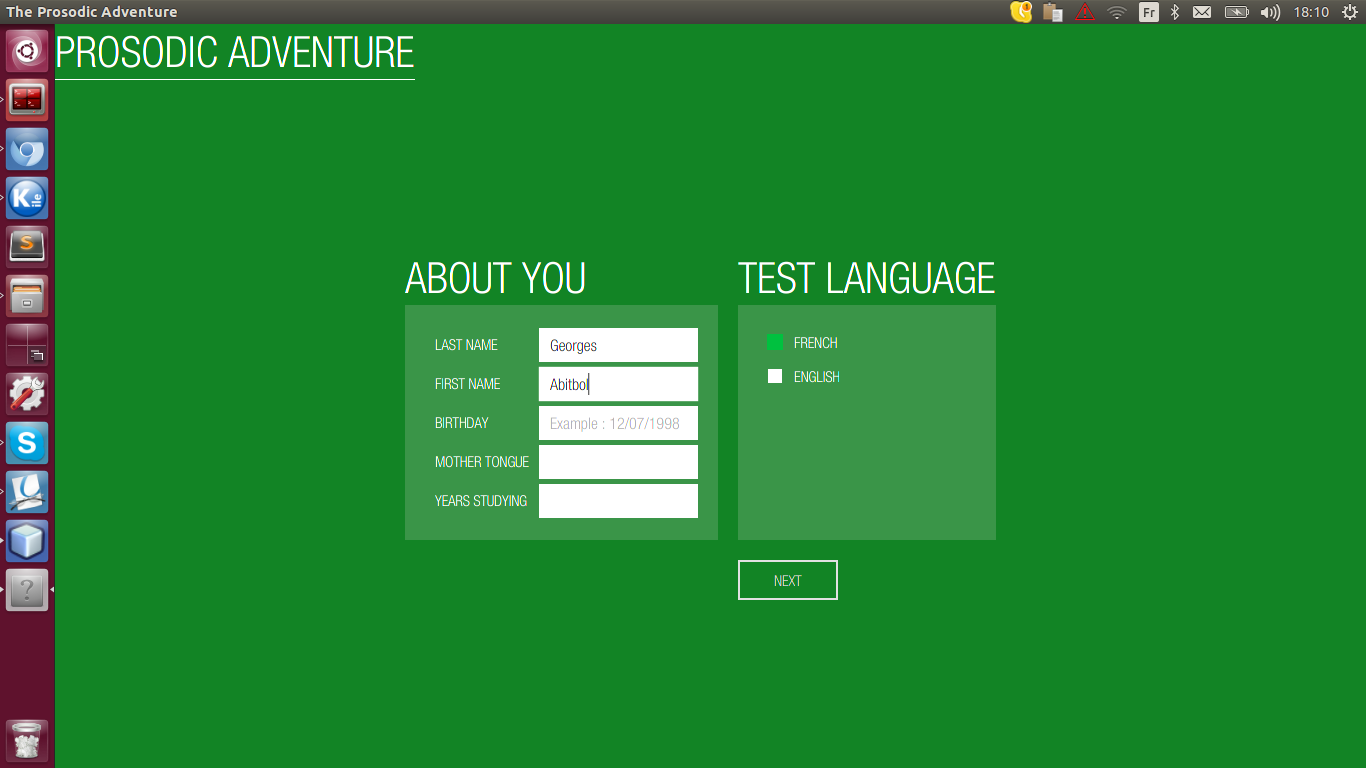
\includegraphics[width=8cm]{./fonctionnement_tests/UserGUI.png}}
  \caption{Fonctionnement - UserGUI}
  \label{diaglog} 
\end{center}
\end{figure}

\subsection{Contrôleur}
\lipsum[7]


\subsection{Exportation des données}
\lipsum[8]